%%%%%%%%%%%%%%%%%%%%%%%%%%%%%%%%%%%%%%%%%%%%%%%%%%%%%%%%%%%%%%%%%%%%%%%%%%%%%%%%%%%%%%%%%%%%%%%%%%%%%%%%%%%%%%%%%%%%%%%%%%%%%%%%%%%%%%%%%%%%%%%%%%%%%%%%%%%%%%%%%%%
% Written By Michael Brodskiy
% Class: Fundamentals of Electromagnetics
% Professor: E. Marengo Fuentes
%%%%%%%%%%%%%%%%%%%%%%%%%%%%%%%%%%%%%%%%%%%%%%%%%%%%%%%%%%%%%%%%%%%%%%%%%%%%%%%%%%%%%%%%%%%%%%%%%%%%%%%%%%%%%%%%%%%%%%%%%%%%%%%%%%%%%%%%%%%%%%%%%%%%%%%%%%%%%%%%%%%

\documentclass[12pt]{article} 
\usepackage{alphalph}
\usepackage[utf8]{inputenc}
\usepackage[russian,english]{babel}
\usepackage{titling}
\usepackage{amsmath}
\usepackage{graphicx}
\usepackage{enumitem}
\usepackage{amssymb}
\usepackage[super]{nth}
\usepackage{everysel}
\usepackage{ragged2e}
\usepackage{geometry}
\usepackage{multicol}
\usepackage{fancyhdr}
\usepackage{cancel}
\usepackage{siunitx}
\usepackage{physics}
\usepackage{tikz}
\usepackage{mathdots}
\usepackage{yhmath}
\usepackage{cancel}
\usepackage{color}
\usepackage{array}
\usepackage{multirow}
\usepackage{gensymb}
\usepackage{tabularx}
\usepackage{extarrows}
\usepackage{booktabs}
\usepackage{lastpage}
\usepackage{float}
\usetikzlibrary{fadings}
\usetikzlibrary{patterns}
\usetikzlibrary{shadows.blur}
\usetikzlibrary{shapes}

\geometry{top=1.0in,bottom=1.0in,left=1.0in,right=1.0in}
\newcommand{\subtitle}[1]{%
  \posttitle{%
    \par\end{center}
    \begin{center}\large#1\end{center}
    \vskip0.5em}%

}
\usepackage{hyperref}
\hypersetup{
colorlinks=true,
linkcolor=blue,
filecolor=magenta,      
urlcolor=blue,
citecolor=blue,
}


\title{Pre-Lab Assignment for Experiment 2}
\date{October 4, 2023}
\author{Michael Brodskiy\\ \small Professor: E. Marengo Fuentes}

\begin{document}

\maketitle

\begin{enumerate}

  \item Given the values for Polyethylene and Polystyrene, a reasonable value for a plastic would probably be somewhere in the low to mid 2-3 range; that is, probably somewhere between $2-2.65$. The dielectric permittivity defines a material's ability to store charge. This means that, given an electric field, the field would be able to permeate some amount of the material, which would store some of that charge. This would mean the charge becomes polarized, which means it aligns with the field.

  \item It seems that, regardless of the value of $Z_n$, the produced graphs remain the same. The voltage and distance remain constant no matter my choice for $Z_n$. Here are some examples:

    \begin{multicols}{2}

      \begin{figure}[H]
        \centering
        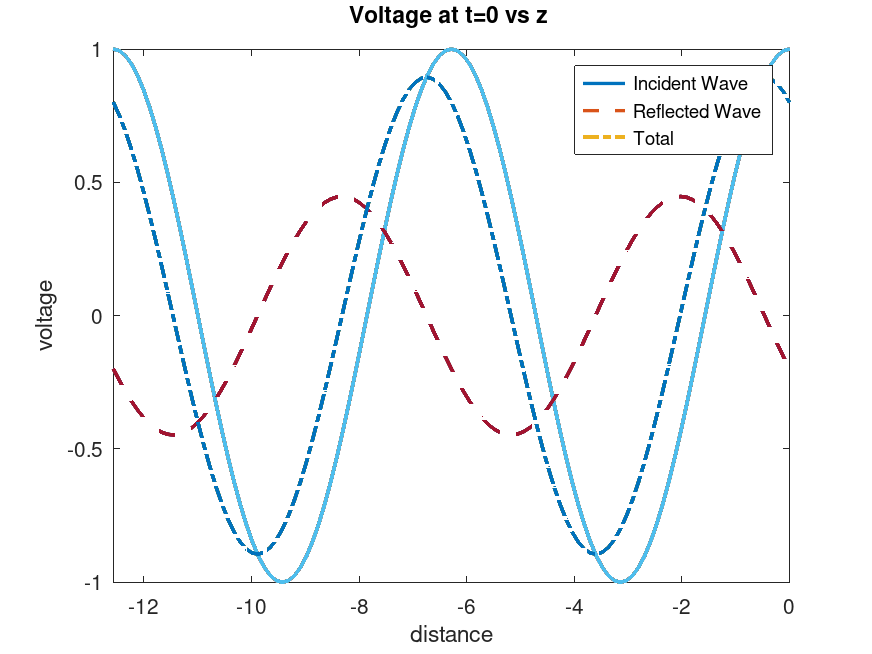
\includegraphics[width=.5\textwidth]{Figures/Lab Two/Zn50.png}
        \caption{$Z_n=50$}
        \label{fig:1}
      \end{figure}

      \begin{figure}[H]
        \centering
        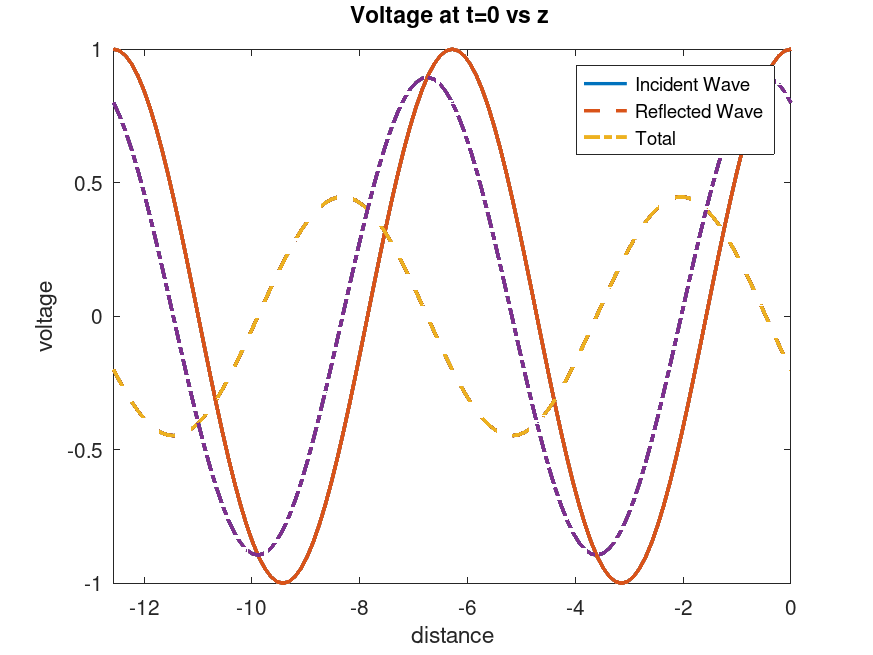
\includegraphics[width=.5\textwidth]{Figures/Lab Two/Zn250.png}
        \caption{$Z_n=250$}
        \label{fig:2}
      \end{figure}

      \begin{figure}[H]
        \centering
        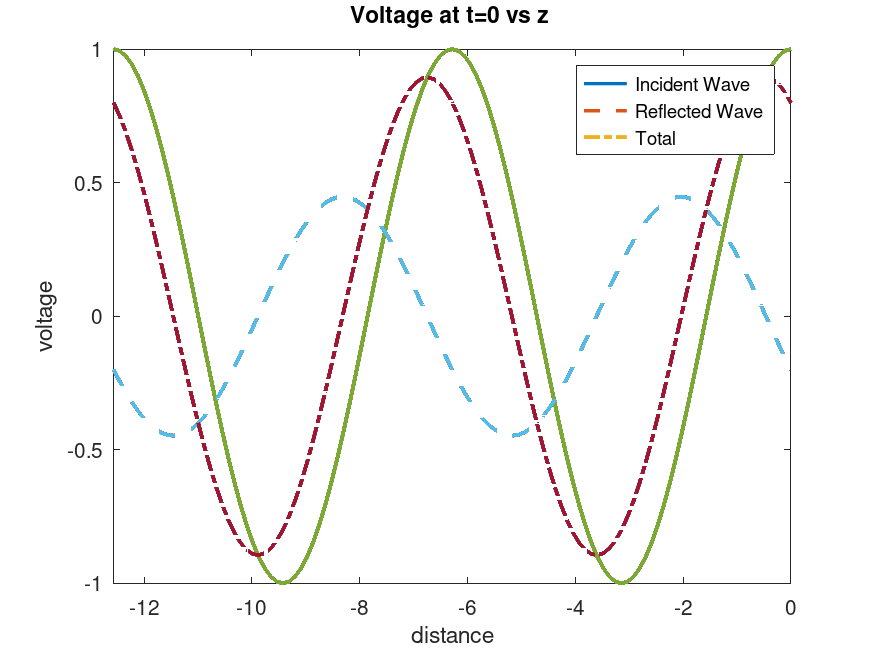
\includegraphics[width=.5\textwidth]{Figures/Lab Two/Zn1k.png}
        \caption{$Z_n=1k$}
        \label{fig:3}
      \end{figure}

      \begin{figure}[H]
        \centering
        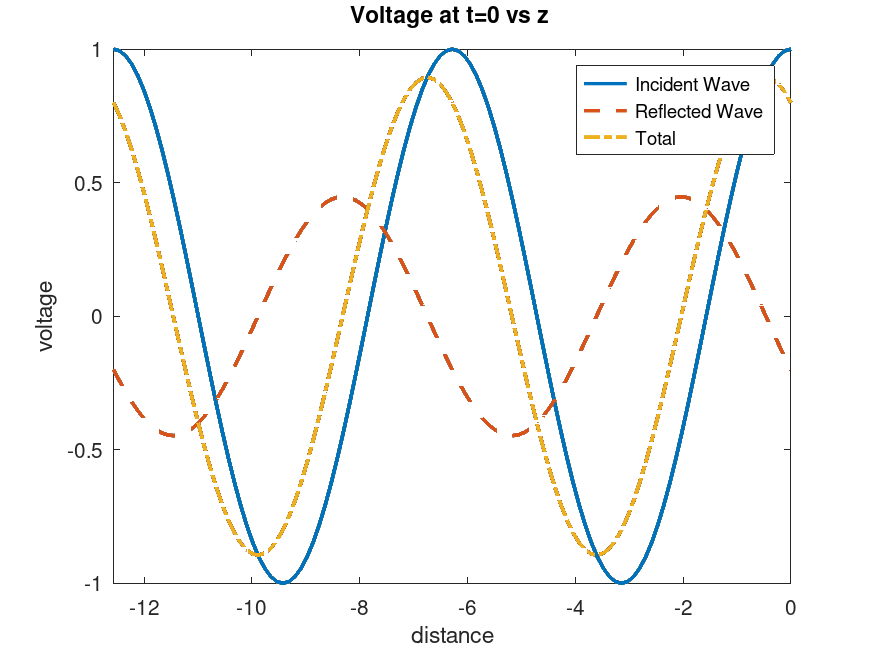
\includegraphics[width=.5\textwidth]{Figures/Lab Two/Zn1M.png}
        \caption{$Z_n=1M$}
        \label{fig:4}
      \end{figure}

      \begin{figure}[H]
        \centering
        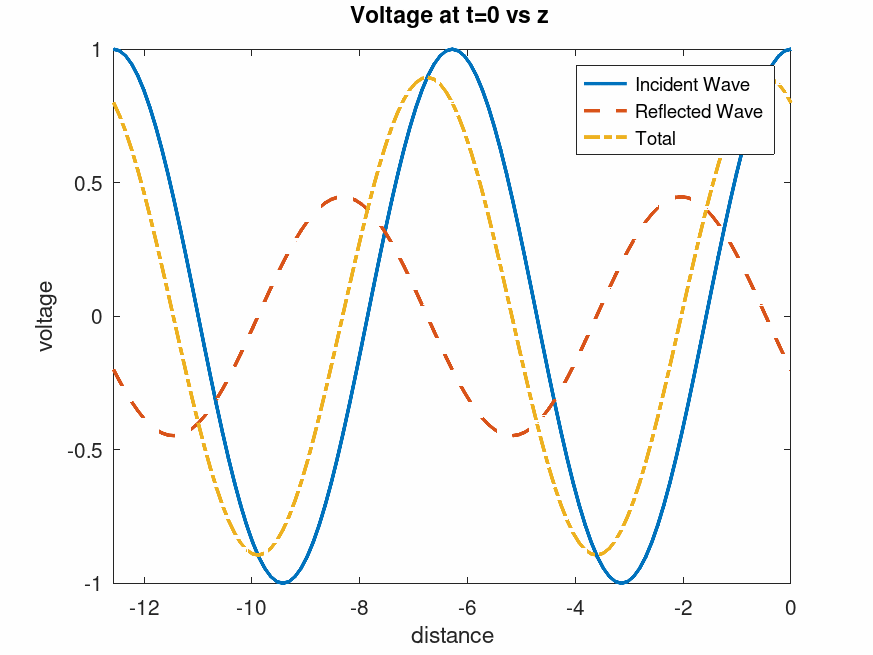
\includegraphics[width=.5\textwidth]{Figures/Lab Two/Zn1-50ki.png}
        \caption{$Z_n=1+50000j$}
        \label{fig:5}
      \end{figure}

      \begin{figure}[H]
        \centering
        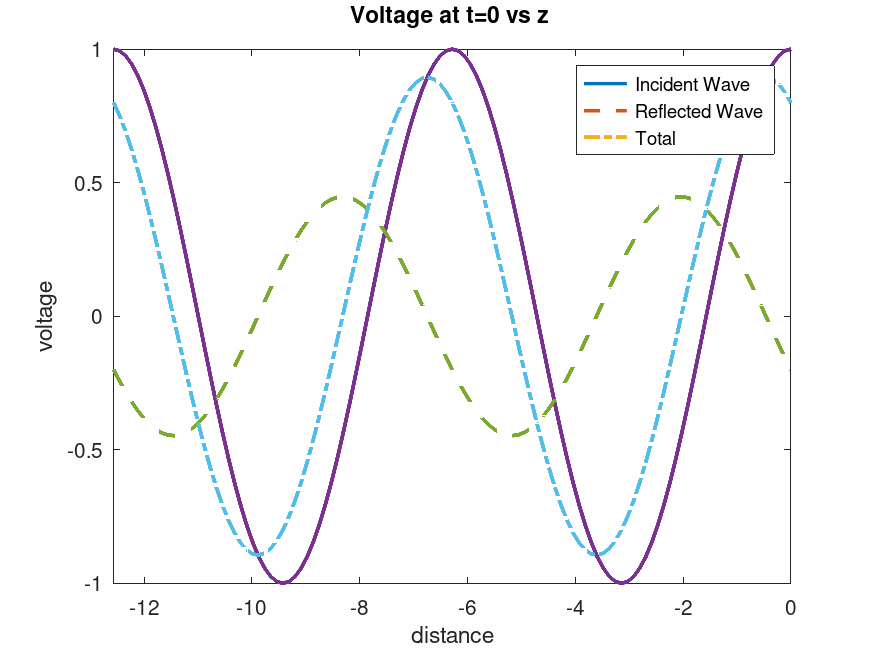
\includegraphics[width=.5\textwidth]{Figures/Lab Two/Zn50k-1i.png}
        \caption{$Z_n=50000+j$}
        \label{fig:6}
      \end{figure}

    \end{multicols}

  \item With the modified code, I can see the wave traveling to the right. It seems that, at $z=-\lambda$, the voltage seems to stay at about 0, no matter what time the wave is at. The overall range does go from approximately $-1$ to $1$, but the voltage is usually always low at $z=-\lambda$.

  \item Assuming a lossless line, constant standing wave ratio circles can be formed. As the length increases, the impedance moves along the constant SWR circles. SWR circles are useful in that they can be used tune impedances to a certain ratio. As the SWR is calculated based on a normalized impedance, the circles can be used to achieve a certain normalized impedance.

\end{enumerate}

\end{document}

